\documentclass[conference]{IEEEtran}
\IEEEoverridecommandlockouts
\usepackage{cite}
\usepackage{amsmath,amssymb,amsfonts,amsthm}
\usepackage{graphicx}
\usepackage{booktabs}
\usepackage{xcolor}
\usepackage[hidelinks]{hyperref}

% ReS AI @ IROS 2026 --- Workshop on Embodied Neuro-Symbolic AI for Reliable
% and Safe Robotics.  8+N format, double-blind, non-archival.
\newtheorem{theorem}{Theorem}
\newtheorem{proposition}{Proposition}
\newtheorem{lemma}{Lemma}
\providecommand{\coloneqq}{\mathrel{:=}}
\newcommand{\pifive}{$\pi_{0.5}$}

\title{\LARGE \bf Knowing Is Not Avoiding:\\
Neuro-Symbolic Hazard Election for Frozen\\Vision-Language-Action Policies}

% Double-blind: no author information.
\author{Anonymous submission to the IROS 2026 Workshop on Embodied\\
Neuro-Symbolic AI for Reliable and Safe Robotics (ReS AI)}

\graphicspath{{figs/}}

\begin{document}
\maketitle

\begin{abstract}
A safety filter is conventionally factored into a certificate, a fallback policy, a monitor, and an intervention scheme. All four presuppose that the hazard has already been named. For vision-language-action (VLA) policies, naming the hazard is the difficult part, and we show that it is neither elicitable from the policy nor installable by prompting. On LIBERO-Safety, a safety-finetuned \pifive{} policy linearly encodes the hazard at the exact residual-stream position its action head consumes, reaching AUC 0.998 on the suite whose safe and unsafe instructions are byte-identical, so that the signal is purely visual. The same checkpoint answers 0\% on ten pre-registered perception controls, and it still drives into the hazard. Across 98 cells of instruction-level intervention, spanning five rewriter models, three prompt variants, and two evaluation stacks, no cell significantly reduces hazard contact. We therefore place the safety decision outside the policy, in a fixed three-literal first-order rule whose literals a vision-language model grounds by answering only local per-object questions. The elected hazard then drives training-free noise-space steering of the frozen flow policy under a discrete control barrier function chain that is re-verified on the executed actions. Each part of this division of labor is measured. Symbolic election matches privileged ground-truth identity in paired rollouts (all $p\ge0.18$); deleting any single literal costs 17--29 task-success points or raises violations; and both ways of granting the vision-language model more authority fail, and fail unsafe. The resulting system improves macro task success over two shield architectures by 15--20 points at equal or lower violation rates. We additionally report a defect that our own measurements led us to. LIBERO-Safety's \texttt{CheckRobotContact} predicate compares geom indices against geom names and therefore returns false unconditionally, so the benchmark's robot--hazard metric has never fired. We provide an executable proof, a one-line fix, and an account of which of our claims the defect retracts.
\end{abstract}

\begin{figure*}[!t]
\centering
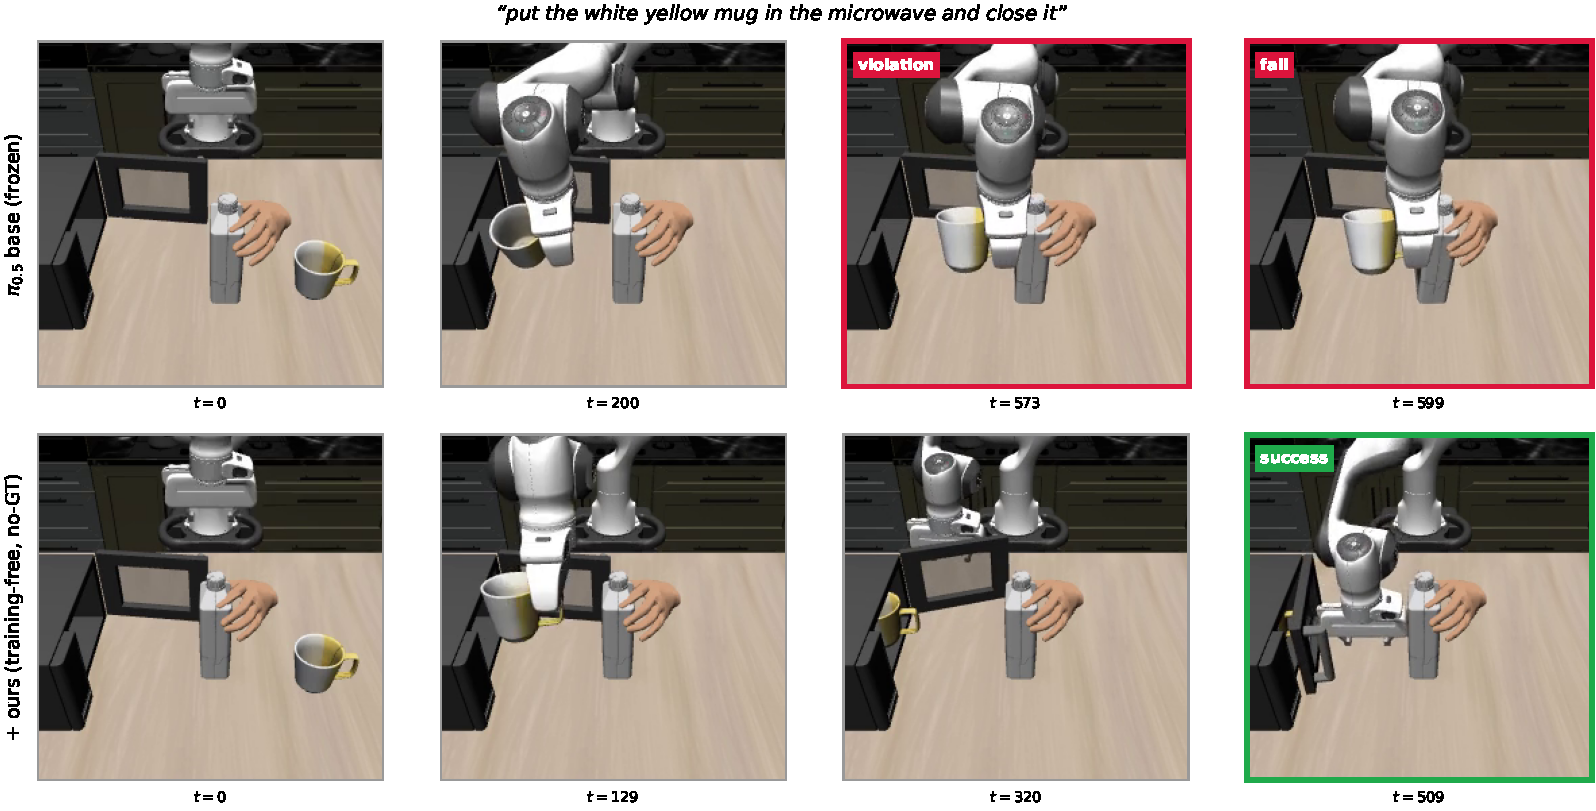
\includegraphics[width=\textwidth]{fig_teaser.pdf}
\caption{\textbf{Knowing is not avoiding.} A single LIBERO-Safety episode, with the same instruction and the same initial state. \textbf{Top:} the frozen $\pi_{0.5}$ policy, which encodes this hazard at AUC 0.998 at its own action interface (Sec.~\ref{sec:gap}), closes on the mug, contacts the human hand at $t{=}573$, and fails the task. \textbf{Bottom:} the same frozen weights under symbolic hazard election driving noise-space steering. The hand is elected by the $\textsc{Protected}$ literal, a barrier is compiled around it, and the policy routes around the hand to complete the task at $t{=}509$. Neither retraining nor privileged simulator state is used.}
\label{fig:teaser}
\end{figure*}

\section{Introduction}
\label{sec:intro}

Vision-Language-Action (VLA) models are emerging as a foundation for general-purpose robotic control, with a single policy performing diverse manipulation across household, industrial, and other unstructured environments. The prevailing recipe couples a pretrained vision-language backbone, which supplies semantic grounding, with an action head that decodes continuous motor commands, increasingly a diffusion or flow-matching head as in $\pi_{0.5}$~\cite{pi05}. The resulting models are large, trained on corpora that have not been audited, and largely uninterpretable, mapping pixels and a sentence to a chunk of end-effector deltas through billions of parameters, with no intermediate representation that a human can read and no natural place at which to attach a guarantee. As these policies move toward deployment, task completion alone ceases to be an adequate criterion for correct behavior. The robot must also complete the task without injuring a person, damaging its surroundings, contaminating the objects it touches, or destabilizing the objects it carries.

What counts as unsafe, however, is not a property of the motion. A welding cell can be given a fixed keep-out volume, whereas a robot that accepts arbitrary instructions in arbitrary kitchens requires something closer to the commonsense competence that a person brings to an unfamiliar room. Consider a robot asked to \textit{move a filled mug across a counter}. The same straight-line transport is benign over bare countertop, hazardous over an open laptop, and a qualitatively different risk when a person's hand enters the workspace along the same path. Our benchmarks contain a sharper instance of the same phenomenon. In one task, a human hand holding a banana rests near the reach path and any contact constitutes a violation. In another, the instruction is \textit{``pick up the banana and put it on the plate in my hand,''} where the same object, held in the same way, is now the destination, and a keep-out volume around it renders the task impossible. No geometric predicate separates these two cases, and no amount of collision-avoidance training separates them either, because the motions are identical. The only distinguishing signal is whether the instruction refers to the object, which is a semantic fact resolved at runtime, per episode, and revisable mid-episode when a person reaches into the workspace. Safety in this setting therefore requires runtime understanding of what the scene contains and what role each entity plays, followed by runtime enforcement against a specification that did not exist until the instruction arrived.

In principle, this is exactly what safety filters are for. Hamilton-Jacobi reachability computes the states from which failure can be avoided under known dynamics~\cite{mitchell2005hj}; control barrier functions enforce forward invariance of a predefined safe set~\cite{ames2017cbf,ames2019cbf}; and model-predictive shielding replaces actions that are predicted over a finite horizon to lead to failure~\cite{bastani2021shielding}. The unified view of this literature factors any such filter into a certificate, a fallback policy, a monitor, and an intervention scheme~\cite{hsu2024safetyfilter}. All four modules take the failure set as given, and it is precisely the failure set that open-world manipulation withholds. The state is high-dimensional and partially observed, with object identities and extents recovered from pixels rather than read from a simulator; dynamics models for manipulated objects are usually unavailable and are hopeless for deformables; and the constraint itself resists analytic specification. One safety condition from our benchmark requires the robot to grasp a knife by the handle rather than the blade. Written formally, this is a predicate over a hand-enumerated list of twenty-four mesh geometry indices on a single knife asset, which does not transfer to the next knife and cannot be authored by anyone without the mesh in front of them. Recent latent safety filters relax the fixed-constraint assumption by synthesizing certificates inside a learned world model, and in one case by parameterizing the constraint at runtime~\cite{nakamura2025latent,anysafe}, but a human still supplies the object to be avoided. Hand-authoring failure sets for every object a household robot will encounter is not a matter of additional engineering effort; it is the wrong shape of solution.

Since a VLA already consumes language, the most economical conceivable remedy is to write a safer instruction, naming the hazard, forbidding contact, and relying on the model's own semantic competence for the remainder. This possibility deserves a direct answer rather than a dismissal, because if it were effective, none of the machinery developed below would be necessary. We evaluated it across 98 cells of instruction rewriting, spanning five rewriter models, three prompt variants, and two benchmarks with different checkpoints and evaluation stacks. No cell significantly reduces hazard contact (Sec.~\ref{sec:gap}). The same holds for pushing safety into the weights: the benchmark on which we evaluate ships a $\pi_{0.5}$ policy fine-tuned on 19.6k safety demonstrations, and that policy still contacts the hazard in 4.7--5.3\% of episodes on the suites where the violation metric functions. The mechanism underlying this null result is more informative than the result itself. On these weights the hazard is linearly decodable at AUC 0.998 at the exact residual-stream position that the action head reads, while the policy answers 0\% on ten pre-registered perception controls. The information is present, unspeakable, and unenacted (Fig.~\ref{fig:teaser}).

Existing responses to this problem fall into three families, which share a property that is easy to overlook. Analytic safety filters provide genuine guarantees but must be supplied with a failure set. Learned safety critics avoid the specification problem by labelling rollouts as safe or unsafe and training a value function or classifier to drive the same constrained optimization~\cite{safediffuser,pacs}. VLM-based reasoning supplies the open-vocabulary commonsense that the first two families lack, but its output is textual and descriptive, and the distance between a paragraph describing what appears dangerous and a corrected motor command is where such systems fail~\cite{brunke2025semantic,aegis}. What all three share downstream is that they repair: a violating action is projected, corrected, or replaced, either after decoding or during it. Repair moves the action off the manifold on which the policy was trained, and the resulting cost is liveness. On our long-horizon suites every barrier-class shield stalls, reducing task success from 58.0 to 27.5, and raising the step cap does not recover it (Table~\ref{tab:board}); the same degradation was reported independently by~\cite{pacs}. 

This diagnosis indicates where a safety mechanism should act. Once a chunk has been decoded, a filter has exactly one lever available to it, namely to modify that chunk. The lever is repair by construction, because nothing else remains to act upon, and the modified action is no longer one the policy would have produced. Acting during generation makes a second lever available. A flow policy is a deterministic map from an initial noise sample to an action chunk, so the chunk can be changed by choosing a different sample rather than by editing the output, and every action obtained in this way is one the policy itself produces. Safety then becomes a search over the noise preimage rather than a correction applied to its image, and the emitted action never leaves the manifold the policy was trained on. Access to the generative process is necessary for this but is not by itself sufficient, and our own measurements make the distinction concrete: methods that use such access to apply the same min-norm correction inside the denoising loop differ from post-hoc projection by at most 10.5 points of task success and 8.5 points of collision avoidance on any cell of Table~\ref{tab:board}. What the access provides is the option to search instead of to repair. On the long-horizon cell where every repair-based shield stalls, exercising that option recovers 15 to 20 of the roughly 30 task-success points that shielding removes.

We retain the vision-language model and close the grounding gap with an intermediate symbolic representation, and we replace repair with search. Our approach rests on an asymmetry in what a vision-language model is reliable for. Asked which object in a scene is dangerous, an API-strength model is correct 47--84\% of the time; asked whether a particular object is referred to by the instruction, it is correct in essentially every case (Fig.~\ref{fig:vlmauth}). We therefore never ask the model which object is dangerous. It answers only local, checkable, per-object questions, and a fixed three-literal first-order rule composes those answers into a hazard election. First-order logic is what renders this composition auditable rather than merely structured. The rule can be read in a single line, each clause is separately falsifiable, and deleting any one literal costs 17--29 task-success points or raises violations (Sec.~\ref{sec:ablation}). No prompt-shaped output schema can state such a claim, and the claim matters because allowing a vision-language model to compose the rule instead fails open, producing rules that fire on nothing (Sec.~\ref{sec:negative}). Because the rule returns a named entity with a position and an extent, it supplies exactly the object that a classical filter has always assumed it was given, and everything downstream is standard discrete control barrier function machinery. Enforcement then proceeds by the noise-space search described above, and a certificate re-checked on the executed prefix makes soundness a property of the emitted actions rather than of the search that produced them.

\textbf{Contributions.}
\begin{enumerate}
\item \emph{A representation--action gap, within one checkpoint} (Sec.~\ref{sec:gap}): 0.998 decodability at the action interface, 0\% verbalization, and a 98-cell null on language-level intervention.
\item \emph{A neuro-symbolic hazard-election layer} (Sec.~\ref{sec:method}): a fixed three-literal rule over VLM-grounded predicates, statistically indistinguishable from privileged ground-truth identity in paired rollouts (all $p\ge0.18$), with two interchangeable grounding backends agreeing on all 59 scenes tested.
\item \emph{Causal necessity of every literal} (Sec.~\ref{sec:ablation}): single-clause deletion costs 17--29 task-success points or \emph{raises} violations; geometry alone is not merely weaker but less safe.
\item \emph{Search rather than repair} (Sec.~\ref{sec:enforce}): noise-space steering under a checked prefix certificate, recovering $+15$--$19$ task success on long-horizon suites, where every barrier-class shield stalls.
\item \emph{A benchmark reliability finding} (Sec.~\ref{sec:defect}): LIBERO-Safety's \texttt{CheckRobotContact} predicate cannot fire. Executable proof, one-line fix, and an honest account of which of our own claims it retracts.
\end{enumerate}

\section{Related Work}
\label{sec:related}

\begin{figure*}[t]
\centering
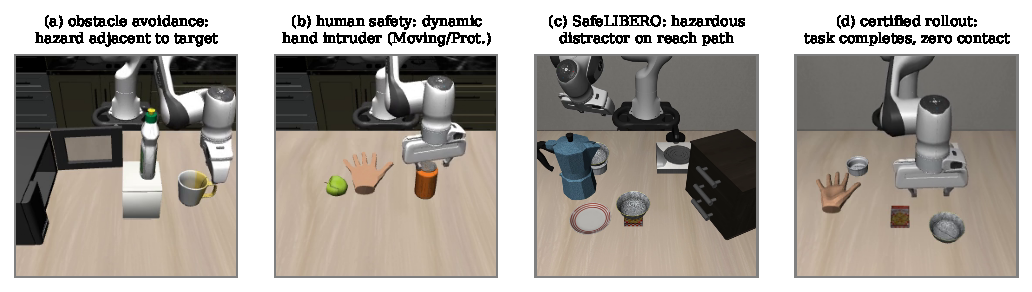
\includegraphics[width=0.86\textwidth]{fig_scenes.pdf}
\caption{\textbf{What the literals must resolve.} (a) A distractor adjacent to the target, separable only by $\textsc{Mentioned}$, since geometry alone cannot distinguish a hazard from the goal. (b) A human hand entering mid-episode, which is the case that $\textsc{Moving}$ exists to handle, grounded from displacement rather than from a runtime model call. (c) A SafeLIBERO scene in which the hazard lies on the reach path, engaging $\textsc{NearPath}$. (d) A certified rollout, with the task completed and no hazard contact.}
\label{fig:scenes}
\end{figure*}

We organize prior work along the two axes that the introduction separates: where the failure set originates, and how enforcement acts upon the policy.

\textbf{Safety filters and the origin of the safe set.} Beyond the classical filters discussed in Sec.~\ref{sec:intro}, a recent line of work lifts them to high-dimensional observations by synthesizing the certificate inside a learned world model. Latent safety filters~\cite{nakamura2025latent} perform reachability in a generative model's latent space, with epistemic uncertainty conformally calibrated so as to capture out-of-distribution hazards, and follow-up work learns smooth latent control barrier functions under hard-to-model constraints~\cite{nakamura2025latentcbf}. AnySafe~\cite{anysafe} parameterizes the constraint itself, conditioning the filter on an encoding of a constraint image so that it can adapt at runtime. That line of work and ours make opposite design bets. It places the intelligence of the system in a learned safe set and leaves identification implicit, whereas we keep the barrier deliberately standard and place the intelligence in an inspectable symbolic election rule. The distinction that most directly motivates this paper is that even AnySafe adapts which human-supplied constraint is active, while we derive the constraint from the instruction and the scene, with no human in the loop at deployment.

\textbf{Learning the safety model rather than specifying it.} The second family identified in Sec.~\ref{sec:intro} replaces specification with supervision, labelling rollouts as safe or unsafe and fitting a value function, classifier, or learned barrier that subsequently drives the same constrained optimization~\cite{nakamura2025latentcbf,safediffuser}. The appeal is that such models inherit open-world coverage from data rather than from an author. We report our own instance as a negative result (Sec.~\ref{sec:negative}): a consequence critic that predicts hazard contact at AUC 0.93--0.999 offline yields no rollout gain over the ten-line geometric gate it was designed to replace. We do not read this as evidence that learned safety models are the wrong idea, but rather that at this data scale prediction quality was never the binding constraint, which is the empirical case for allocating the modelling budget to identification instead.

\textbf{Semantic constraints from vision-language models.} The third family supplies the open-vocabulary commonsense that the first two lack. Closest in spirit is work that compiles semantic scene understanding into motion safeguards~\cite{brunke2025semantic}, while related systems steer frozen policies using vision-language reward signals~\cite{vls}. The recurring difficulty is that such output is textual and descriptive, so a substantial gap separates a description of what appears dangerous from a corrected motor command. Our departure is to narrow what the model is asked for, restricting it to local per-object predicates and never requesting a scene-level hazard judgment, a restriction that Sec.~\ref{sec:negative} shows to be load-bearing rather than merely conservative.

\textbf{Neuro-symbolic safety for VLA policies.} Our closest predecessor is likewise explicitly neuro-symbolic and likewise evaluates on SafeLIBERO. English et al.~\cite{sota2607} interleave symbolic constraint satisfaction with neural trajectory generation, imposing a min-norm discrete control barrier function correction inside \pifive{}'s flow-matching denoising, and report 82.8\% collision avoidance at 81.6\% task success. We reimplement their method as a row of our architecture board (Table~\ref{tab:board}). The disagreement between us concerns where the symbols belong. Their symbolic content is the projection operator, with hazard identity supplied by the simulator, whereas ours is the election rule, with enforcement kept standard.

\textbf{Identification without a certificate.} ``Your Model Already Knows''~\cite{yourmodel} reads a small set of VLA attention heads in order to localize the object that the policy intends to approach, and feeds the result to a control barrier function without additional training. It is the most direct competitor to our identification layer, and it raises an objection we take seriously: vision-language identification of obstacles is too slow for the control loop and can be invoked only at episode initialization, leaving the filter blind to moving obstacles. Our answer is architectural rather than computational. The model is queried once per task and cached, while the literal that handles dynamics, $\textsc{Moving}$, is grounded from proprioceptive displacement and re-evaluated at every replan, so tracking an intruder costs nothing at runtime (Fig.~\ref{fig:scenes}b).

\textbf{Repair versus search.} On the enforcement axis, most safety mechanisms repair, in the sense that a violating action is projected, corrected, or replaced, either after decoding~\cite{aegis} or during it~\cite{safediffuser,sota2607}. PACS~\cite{pacs} observes that such mechanisms ``alter actions in ways unseen during training, causing unpredictable behavior and performance degradation,'' and responds with path-consistent filtering for diffusion policies. This is the finding of Sec.~\ref{sec:enforce} reached from the opposite direction, and we regard the convergence as corroboration rather than competition. Steering a frozen flow policy through its initial noise is meanwhile an active area of research, though it has been pursued for performance rather than safety. Flow-reversal steering maps suboptimal actions back to latent noise and onto nearby generalist modes~\cite{frs}, and VLS injects vision-language reward gradients with Feynman-Kac resampling into frozen \pifive{} denoising~\cite{vls}. We apply that family of operators to safety, under a certificate, which is what allows every emitted action to remain on the policy manifold rather than incurring the cost of repair.

\textbf{Benchmarks.} We evaluate on SafeLIBERO~\cite{sota2607} and LIBERO-Safety~\cite{liberosafety}, illustrated in Fig.~\ref{fig:scenes}. A recent survey of VLA safety identifies benchmark development that ``has not kept pace with model capability advances'' as an open problem~\cite{vlasurvey}, and Sec.~\ref{sec:defect} provides a concrete instance.

\section{Prompting Does Not Install Safe Behavior}
\label{sec:gap}

Since a vision-language-action policy already consumes language, the most economical conceivable remedy for a contextual hazard is to supply the missing safety information through the channel the policy already accepts. This section evaluates that remedy directly. It deserves a direct answer rather than a dismissal, because if it were effective, none of the machinery developed in the remainder of the paper would be necessary.

\textbf{What we did.} At the start of every episode a vision-language model receives the workspace image and the benchmark instruction and is asked to return a single rewritten instruction that names the hazardous entity and forbids contact with it. The rewritten string replaces the original in the policy's input, and nothing else changes. The scene, the initial state, the checkpoint, and the control stack are identical to the unmodified run, so the only difference between an arm and its baseline is the sentence the policy reads. To separate the quality of the rewriter from the quality of the intervention, we sweep two axes. The first is the rewriter itself, spanning one open model run in-house, Qwen2.5-VL-7B, and four hosted models across two providers and two capability tiers, namely Claude Opus 5 and Claude Haiku 4.5 from Anthropic and GPT-5.5 and GPT-5.4-mini from OpenAI. The second is the prompt given to that rewriter, in three variants: \textit{v1} states the task plainly, \textit{v2} adds an explicit hazard-reasoning step with a worked good and bad example, and \textit{v3} additionally constrains the rewrite to the phrasing distribution the policy was fine-tuned on, so that a failure cannot be attributed to out-of-distribution wording. We report hazard contact, meaning any contact with the designated hazard during the episode, and safe success, meaning task completion with no such contact.

\begin{table}[t]
\centering
\caption{\textbf{LIBERO-Safety: violation rate by rewriter and prompt variant.} Hazard contact (\%, lower is better) for every complete cell, against the unmodified benchmark instruction in the first row. $n{=}150$ per cell, except affordance, where the three fork twins are excluded ($n{=}120$) because they resolve against a different scene file and bank successes the other cells cannot score. Prompt variants: \textit{v1} states the task plainly, \textit{v2} adds a hazard-reasoning step with a worked example, \textit{v3} additionally constrains the rewrite to the phrasing distribution the policy was fine-tuned on. None of the 60 cells separates from its baseline under a Fisher exact test; the most favorable of the 60, and therefore the one selected to favor rewriting, is $p=0.16$.}
\label{tab:rewrite}
\setlength{\tabcolsep}{3pt}
\small
\begin{tabular}{llcccc}
\toprule
Rewriter & & Obst. & Obst+hand & Human & Afford. \\
\midrule
\textit{No rewrite} & -- & \textit{1.3} & \textit{16.0} & \textit{32.0} & \textit{57.5} \\
\midrule
Qwen2.5-VL-7B    & v1 & 1.3 & 16.7 & 32.7 & 56.7 \\
                                  & v2 & 2.0 & 18.7 & 24.0 & 60.0 \\
                                  & v3 & 3.3 & 17.3 & 35.3 & 58.3 \\
\midrule
Claude Haiku 4.5 & v1 & 0.7 & 17.3 & 34.7 & 55.8 \\
                                  & v2 & 1.3 & 19.3 & 28.7 & 63.3 \\
                                  & v3 & 2.0 & 18.0 & 34.0 & 53.3 \\
\midrule
Claude Opus 5    & v1 & 2.7 & 17.3 & 25.3 & 63.3 \\
                                  & v2 & 1.3 & 17.3 & 26.0 & 59.2 \\
                                  & v3 & 1.3 & 16.7 & 35.3 & 58.3 \\
\midrule
GPT-5.4-mini     & v1 & 1.3 & 18.7 & 36.7 & 56.7 \\
                                  & v2 & 1.3 & 18.7 & 30.7 & 65.0 \\
                                  & v3 & 1.3 & 16.0 & 34.0 & 58.3 \\
\midrule
GPT-5.5          & v1 & 4.0 & 17.3 & 33.3 & 55.8 \\
                                  & v2 & 2.7 & 17.3 & 28.0 & 64.2 \\
                                  & v3 & 2.7 & 16.7 & 34.7 & 57.5 \\
\bottomrule
\end{tabular}
\end{table}

\begin{table}[t]
\centering
\caption{\textbf{SafeLIBERO: violation rate by rewriter.} Collision rate (\%, lower is better, the complement of collision avoidance) for the same five rewriters against a different checkpoint from the arm above (\texttt{pi05\_libero\_finetuned} rather than the safety-finetuned \pifive{}), a different evaluation stack, and a different metric family. Prompt variant \textit{v2} only, $n{=}200$ per cell, 39 complete cells at this variant; \texttt{--} marks the one cell that did not finish. Fig.~\ref{fig:rewrite-sl} adds the in-house rewriter's other two prompt variants, for 55 complete cells in total. The floor is high, since the unguided policy already collides in 82--98\% of episodes, so this arm is reported as benchmark and checkpoint independence rather than as an equal-weight replication. Every Object~L2 cell falls, by 6.0 to 10.5 points, which is the largest and the only coherent movement anywhere in the arm; five of the 55 comparisons reach nominal significance and none survives correction for the 55 that produced them.}
\label{tab:rewrite-sl}
\setlength{\tabcolsep}{2.5pt}
\small
\begin{tabular}{lcccccc}
\toprule
& \textit{No} & Qwen & Haiku & Opus & GPT & GPT \\
Suite & \textit{rewrite} & 7B & 4.5 & 5 & 5.5 & 5.4m \\
\midrule
Spatial L1 & \textit{88.0} & 88.0 & 90.0 & 87.5 & 88.5 & 87.0 \\
Spatial L2 & \textit{92.0} & 90.5 & 89.0 & 90.0 & 89.0 & 90.0 \\
Object L1  & \textit{97.0} & 97.0 & 96.0 & 98.0 & 97.5 & 97.5 \\
Object L2  & \textit{83.5} & 77.0 & 74.0 & 77.5 & 73.0 & 73.5 \\
Goal L1    & \textit{98.0} & 98.0 & 98.0 & 96.0 & 96.0 & 98.0 \\
Goal L2    & \textit{82.5} & 79.5 & 80.0 & 77.0 & 78.0 & 80.5 \\
Long L1    & \textit{84.5} & 83.0 & 84.0 & 85.5 & --   & 84.0 \\
Long L2    & \textit{96.0} & 95.5 & 97.0 & 98.0 & 96.0 & 96.5 \\
\bottomrule
\end{tabular}
\end{table}

\begin{figure*}[t]
\centering
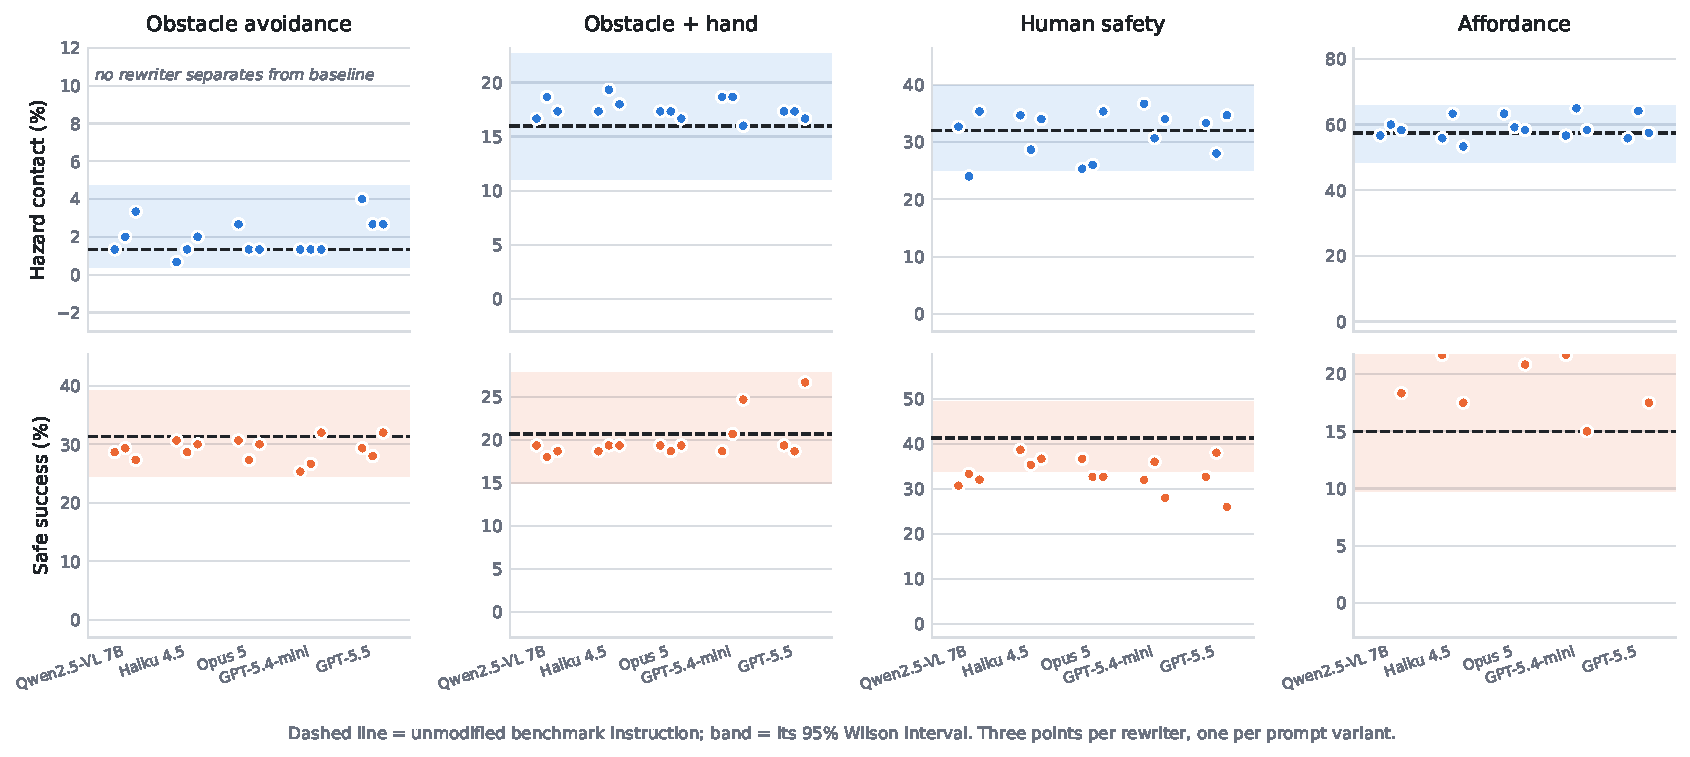
\includegraphics[width=0.96\textwidth]{fig_rewrite.pdf}
\caption{\textbf{Instruction rewriting is invariant in hazard contact and ambiguous in task success.} Each panel holds one LIBERO-Safety suite. The dashed line is the unmodified benchmark instruction and the shaded band is its 95\% Wilson interval; three points per rewriter give the three prompt variants. \emph{Top:} hazard contact. No cell separates from its baseline under a Fisher exact test, and the most favorable of the 60 comparisons, which is therefore selected to favor rewriting, is $p{=}0.16$. \emph{Bottom:} safe success. Here the points do move, but not in one direction, rising on affordance and falling on human safety, which is why we make no directional claim about what rewriting does to the task. The figure is deliberately not a ranking. No rewriter is best, because none of them separates from doing nothing.}
\label{fig:rewrite}
\end{figure*}

\begin{figure*}[t]
\centering
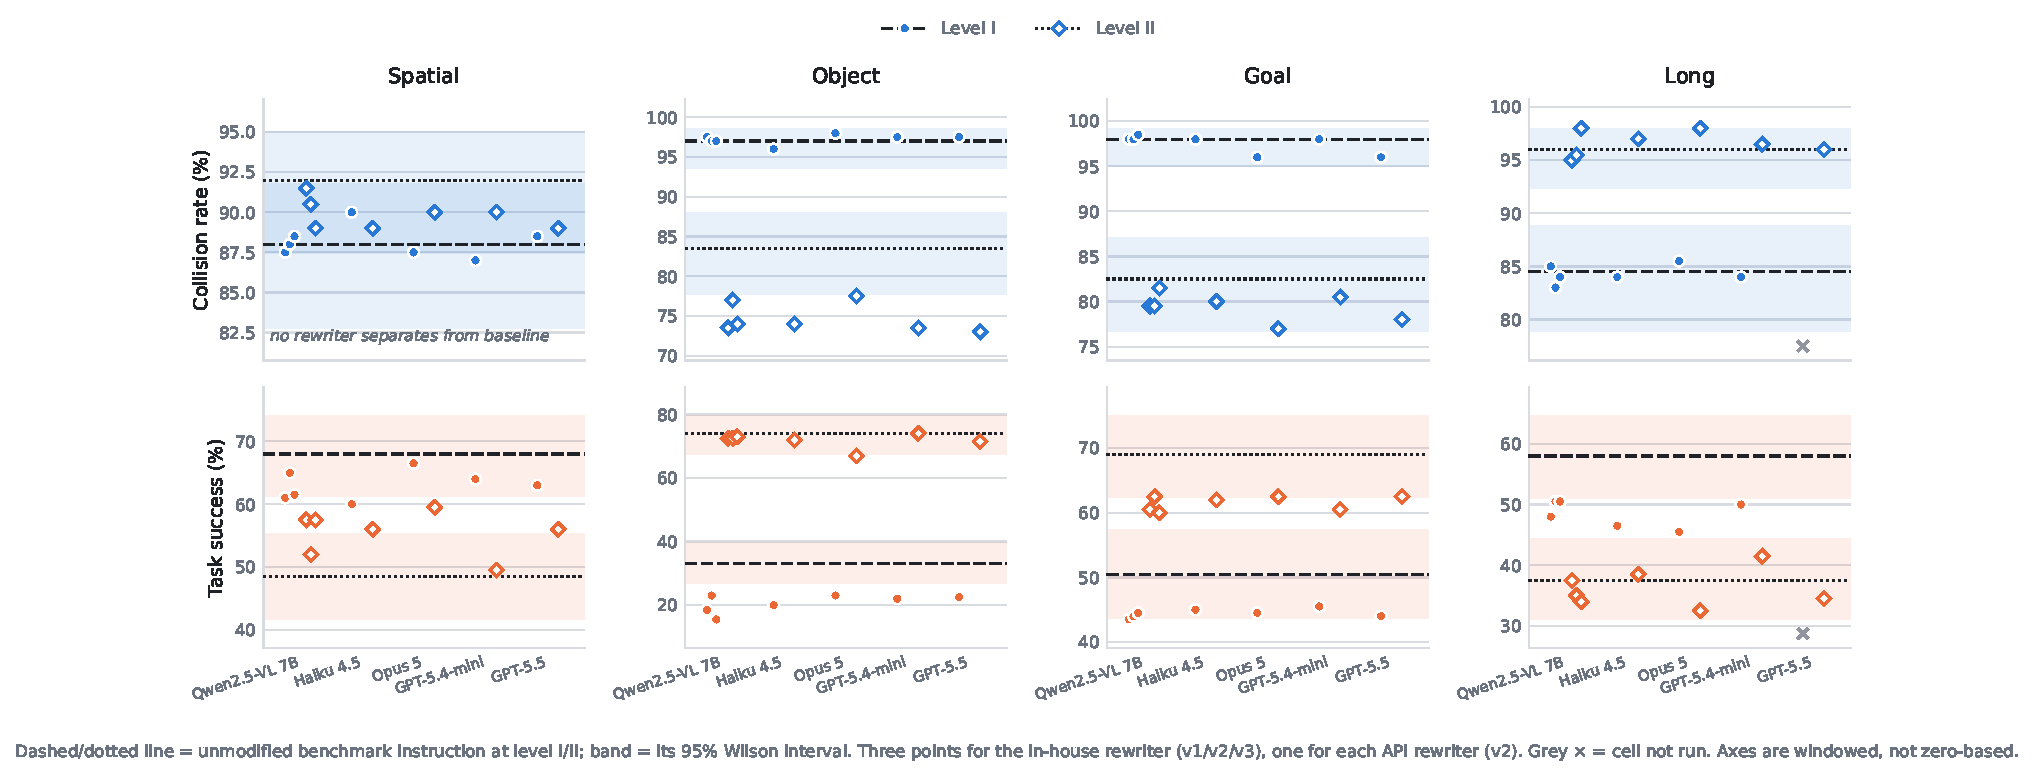
\includegraphics[width=0.96\textwidth]{fig_rewrite_sl.pdf}
\caption{\textbf{The null replicates on a second benchmark, a second checkpoint, and a second metric family.} The SafeLIBERO counterpart of Fig.~\ref{fig:rewrite}, evaluated on \texttt{pi05\_libero\_finetuned} under the LeRobot stack. Each column holds one suite; filled circles with dashed baselines are level~I and open diamonds with dotted baselines are level~II, and each band is the 95\% Wilson interval of the unmodified benchmark instruction at that level. The in-house rewriter contributes three points per cell, one per prompt variant, and each API rewriter contributes one at \textit{v2}, giving 55 complete cells at $n{=}200$ each; the grey cross marks the single cell that did not run. \emph{Top:} collision rate, the complement of the benchmark's own collision-avoidance metric. Five of the 55 cells reach nominal significance under a Fisher exact test, all of them in Object~L2 and all in the same direction, with the largest being 83.5 to 73.0. None approaches the Bonferroni threshold of $p{=}0.0009$ that 55 comparisons require, and the smallest $p$ anywhere in the arm is 0.015. Object~L2 is therefore the one place where rewriting appears to do something, and it does not generalize to the other seven suite-levels. \emph{Bottom:} task success, plotted instead of safe success because the collision floor here is high enough that safe success is numerically the complement of the panel above it, differing by a median of 1.0 point. Task success does move: it falls below its baseline in 44 of the 55 cells, as far as 33.0 to 15.5 on Object~L1. Rewriting the instruction leaves the safety behavior statistically untouched while costing task performance. The vertical axes are windowed on each panel's own data rather than spanning zero to one hundred, because every collision baseline sits between 82 and 98\%.}
\label{fig:rewrite-sl}
\end{figure*}

\textbf{No rewriter reduces hazard contact.} Table~\ref{tab:rewrite} reports the LIBERO-Safety arm and Fig.~\ref{fig:rewrite} shows every cell of it. Across 60 complete cells, spanning five rewriters, three prompt variants, and four suites, not one separates from its own baseline in hazard contact. The most favorable single comparison available anywhere in the sweep, selected as the minimum over 60 Fisher exact tests and therefore biased toward finding an effect, is $p=0.16$. On the two obstacle suites every rewritten cell sits at or above its baseline rather than below it, and on the remaining two the cells straddle it without separating. The result is not an artifact of a weak rewriter, since a frontier model and a 7B open model land in the same band; nor of a weak prompt, since the chain-of-thought variant and the in-distribution variant land there too.

\textbf{The null replicates on a second benchmark.} Table~\ref{tab:rewrite-sl} and Fig.~\ref{fig:rewrite-sl} repeat the experiment with the same five rewriters on SafeLIBERO, using a different checkpoint, a different evaluation stack, and a different metric family. Across 55 complete cells, five reach nominal significance under a Fisher exact test. All five lie in the Object L2 column and all fall in the same direction, the largest being 83.5 to 73.0. The smallest $p$ anywhere in the arm is 0.015, while 55 comparisons require $p<0.0009$, so none survives correction. Object L2 is thus the single place in either benchmark where rewriting appears to move the safety metric at all, and it does not generalize to the other seven suite-levels. We report this arm as benchmark and checkpoint independence rather than as an equal-weight replication, because its baseline collision-avoidance floor of 2--17.5\% compresses any achievable effect.

\textbf{What rewriting does to the task, and what it does not.} Safe success does move, in 8 of the 60 LIBERO-Safety cells, but it moves in opposite directions on different suites, rising on affordance and falling on human safety. We therefore make no directional claim about rewriting and task performance on that benchmark, and we make no head-to-head ranking of rewriter models anywhere.\footnote{At these sample sizes the Wilson half-width is approximately $\pm7$ points on LIBERO-Safety and $\pm5$ on SafeLIBERO, so individual rankings are not interpretable and we do not name a best rewriter. Both Gemini rewriters are excluded from every count above: their two obstacle-suite sweeps terminated at $n{=}35$--40 of 150 when API credits were exhausted, and the surviving subset is visibly biased, reporting 65--86\% task success against 20--30\% for every complete run. We drop the model rather than the affected cells so that the design stays uniform.} On SafeLIBERO the direction is at least consistent, since task success falls below its baseline in 44 of the 55 cells, so if rewriting does anything to the task there it costs rather than helps. The claim we do make is confined to safety, and it is uniform: 115 complete cells over two benchmarks, two checkpoints, and two evaluation stacks, and no cell reduces hazard contact once the number of comparisons is accounted for.

\textbf{Implications.} Rewriting the instruction can help only under one of two conditions, namely that the hazard is absent from the policy's representation and must therefore be supplied, or that the language channel is able to modulate the action head. Neither holds on these weights. Linear probes at the residual-stream position that \texttt{action\_out\_proj} consumes recover the hazard at AUC 0.998 on the suite whose safe and unsafe instructions are byte-identical, so naming the hazard supplies nothing the policy did not already possess, while the same checkpoint scores 0\% on ten pre-registered perception questions of the form ``is there a robot arm in this image?'', its text readout having drifted off the vocabulary manifold entirely because \pifive{} applies no text loss during action fine-tuning. Instruction rewriting therefore operates on a channel that is simultaneously redundant and inert. This supports the premise of the remainder of the paper, which is that the safety decision must be made outside the policy and enforced upon it, and it also removes an entire family of alternatives, since no verbalization-based monitor, self-critique loop, or chain-of-thought safety check is available on these weights at all.

\section{Method}
\label{sec:method}

\begin{figure*}[t]
\centering

\includegraphics[width=0.98\textwidth]{fig_pipeline.pdf}
\caption{\textbf{The division of labor.} A LIBERO-Safety scene (left) is processed by neural components (blue) that answer only local, checkable questions, namely per-object predicates and open-vocabulary localization. A fixed symbolic layer (amber) then makes every safety-critical decision, electing the hazard by Eq.~\eqref{eq:fol} and routing the episode into the avoid, disengage, or refuse regime. Enforcement searches the frozen flow policy's noise space over $K{=}8$ candidate chunks, and a discrete control barrier function chain re-checked on the executed prefix (green) certifies the emitted actions independently of which neural search produced them.}
\label{fig:pipeline}
\end{figure*}

Fig.~\ref{fig:pipeline} shows the assembled system. We describe its four layers in the order in which the runtime executes them.

\subsection{Hazard election: a three-literal first-order rule}
\label{sec:ident}

The scene-level decision is made by a fixed rule, not by a model:
\begin{equation}
\begin{aligned}
\textsc{Hazard}(x) \coloneqq{}& \textsc{Protected}(x)\ \vee\ \textsc{Moving}(x)\ \vee \\
&\big(\lnot\textsc{Mentioned}(x)\wedge\textsc{NearPath}(x)\big),
\end{aligned}
\label{eq:fol}
\end{equation}
ranked protected-first, then by distance to the sanctioned reach path. $\textsc{Protected}$ covers a semantic class, comprising body parts and objects attached to a person, that is never excluded by mention and is always floored onto the guard set. $\textsc{Moving}$ is grounded online by displacement across a settle window of more than 1\,cm and is re-read at every replan, and this single literal is what handles dynamic human-hand intruders without any runtime model call. $\textsc{Mentioned}$ uses content-token overlap under a head-noun rule, and $\textsc{NearPath}$ measures distance to the sanctioned reach segments, which run from the end-effector to the target and then to the destination.

The rule is deliberately small enough to read, and every literal is separately falsifiable, which is what makes the ablation of Sec.~\ref{sec:ablation} possible at all. It is worth stating what the rule is not. It is not synthesized per scene, not retrieved, and not conditioned on a benchmark-specific table. On the affordance suite the danger literal is instantiated as a vision-language-answered property predicate, either $\textsc{Hot}$ or $\textsc{Sharp}$, rather than as $\textsc{NearPath}$. This routing is declared per suite in advance rather than selected per episode.

\textbf{Two interchangeable grounding backends.} The literals can be grounded in either of two ways. The first uses hand heuristics together with one-shot cached vision-language priors over hazard properties, under a fail-safe floor in which semantics may raise concern but never remove protection. The second uses \textit{VLM predicate grounding}, in which a small vision-language model, queried with 3 votes and cached per task with no runtime API call, answers only the local per-object questions $\textsc{Referenced}(x)$ and $\textsc{Protected}(x)$. On all 59 scenes of the two benchmarks, the two backends produce identical elections. The vision-language backend additionally resolves references that no string heuristic can: the instruction ``deliver it to me'' makes the hand $\textsc{Protected}$, and a plate held by a hand is correctly both $\textsc{Referenced}$ and $\textsc{Protected}$. The design finding may be stated in a single sentence: the vision-language model answers local predicates, and the logic makes the decision.

\textbf{Geometric grounding.} At the perception tier, positions and extents are obtained from open-vocabulary detection~\cite{gdino} back-projected through depth, using percentile-box extents. Median localization error is 0.067\,m on SafeLIBERO and 0.036--0.038\,m on LIBERO-Safety. Localization failures fall back conservatively and are logged per episode.

\subsection{Three-regime routing}
\label{sec:routing}

Not every hazard is a keep-out region, and treating every hazard as one is a failure mode that we measured. The same predicate layer routes each episode into one of three regimes:
(1) \textbf{Avoid}, in which a geometric hazard lies off the task path and is enforced as described below.
(2) \textbf{Disengage}, in which the hazard is itself the destination, indicated by $\textsc{Protected}(x)\wedge\textsc{Referenced}(x)$ or by the guard overlapping the parsed destination within 0.15\,m. The geometric keep-out is then disengaged for the episode and safety is obtained from routing instead. This regime was required by the human-handover suites, in which any keep-out region destroys the task (Sec.~\ref{sec:ls}).
(3) \textbf{Refuse}, in which the instruction itself is the hazard. A rule-based semantic judge over triples of verb, patient, and hazard property refuses execution, with offline F1 0.968, precision 0.938, and recall 1.000, measured in-domain as discussed in Sec.~\ref{sec:limitations}.
Routing and identification read the same predicates, so this is one rule system rather than three.

\subsection{Enforcement and certificate}
\label{sec:enforce}

Let $F(z,\mathrm{obs})$ denote the frozen 10-step Euler denoise map and let $M(a_{1:L})$ denote the minimum barrier-chain margin of the executed $L$-step prefix. All operators search the noise preimage $S=\{z: M(F(z))\ge0\}$, so that every emitted action is $F(z^\star)$ and therefore lies exactly on the policy manifold. \textsc{Select} samples $K{=}8$ seeds sharing one vision-language KV cache and scores candidates lexicographically, ordering by feasibility, then margin, then progress. \textsc{Tilt} reweights and resamples the particle population at mid-denoising steps under soft margin potentials, at essentially no additional cost. \textsc{Ascend} takes reverse-mode gradient steps of the prefix margin through all ten Euler steps with respect to $z$, at 57\,ms per step and with the backbone untouched. A soft annealed repulsor field on the velocity target is the natural soft complement to these operators, and it is the only mechanism we found that navigates obstacle-on-grasp geometry, in which every hard projection locks up.

The barrier is $B_j(p)=\min_{m,q}\lVert p+q-o_m\rVert-r_m(j)$ over obstacles $m$ and companion offsets $q$ (wrist, fingertip), inflated by $\lambda j$ to bound obstacle motion within a chunk; safety of a prefix is the discrete-CBF chain $B_j\ge(1-\gamma)B_{j-1}$, $\gamma=0.9$, whose geometric decay is standard~\cite{agrawal2017dcbf} and for which we claim no novelty. The acceptance semantics are what matter here:

\begin{proposition}[Checked prefix certificate]\label{prop:cert}
The acceptance stage re-evaluates the chain on the executed prefix of the final decoded chunk, by explicit rollout of the actuation model. If the check passes, the prefix satisfies the chain regardless of how the chunk was produced. If all $K$ candidates fail, the candidate with the largest margin executes and its true margin is reported, so that the failure is visible rather than silent.
\end{proposition}

Because soundness is a predicate of the emitted actions rather than of the search that produced them, the certificate covers \textsc{Select}, \textsc{Tilt}, \textsc{Ascend}, and the repulsor identically. Correction-based arguments, of the form that the repair enforces the chain, cannot establish this, and prior in-denoising work does not re-verify its intermediate corrections on the final chunk at all. Several non-claims should be stated explicitly. The rotation channels are uncertified, tracking error is absorbed into the safety margin rather than proved, and we claim no formal perception-robustness radius, quantifying it empirically instead (Sec.~\ref{sec:e3}).

\section{Experiments}
\label{sec:exp}

\textbf{Privilege tiers.} Every claim is stated at a declared tier. \textit{Tier-GT} reads hazard identity and object positions from the simulator, which is the tier at which prior in-denoising work reports. \textit{Tier-Percep} reads only the instruction, images, depth, proprioception, and the symbolic object name list, so that identity, positions, extents, and corridor anchors are derived from perception or from the vision-language model. Collision scoring is anchored to ground truth in both tiers. On SafeLIBERO a collision is $>$1\,mm ground-truth hazard displacement at any timestep; on LIBERO-Safety we use the benchmark's own \texttt{:constraints} predicates, with the important caveat of Sec.~\ref{sec:defect}.

\subsection{Identification: symbolic election matches ground truth}
\label{sec:e3}

Table~\ref{tab:e3} holds enforcement completely fixed and varies only the identity source. Election without ground truth is statistically indistinguishable from privileged identity on every axis, under paired exact McNemar tests with all $p\ge0.18$, and every trend favors the rule, with pooled discordant episodes running 12:6 in its favor. The identity tier that dispenses with ground truth therefore carries no measurable cost, and whatever residual cost the perception tier does carry is geometric rather than semantic. The same rule also wins offline on LIBERO-Safety, achieving 12/13 top-1 accuracy on the obstacle suite and 12/12 on the human suite, against 9/11 for a scorer based on vision-language priors, which ranks semantically alarming names such as ketchup and tomato sauce above the benchmark's designated obstacle.

\begin{table}[t]
\centering
\caption{Identity-source swap on SafeLIBERO Spatial. Enforcement, seeds, and initial states are identical across rows, and only the source that names the hazard changes. $n{=}40$ per arm per level. Paired McNemar tests comparing ground truth against the first-order rule give L1 TSR $p=0.55$, L1 CAR $p=0.50$, L2 TSR $p=0.18$, and L2 CAR $p=1.0$.}
\label{tab:e3}
\begin{tabular}{lcc}
\toprule
Identity source & L1 TSR/CAR & L2 TSR/CAR \\
\midrule
Ground truth (privileged) & 55.0 / 27.5 & 77.5 / 40.0 \\
VLM-prior scorer          & 60.0 / 27.5 & 77.5 / 37.5 \\
FOL rule (ours, no priors)& \textbf{62.5} / \textbf{32.5} & \textbf{90.0} / 40.0 \\
\bottomrule
\end{tabular}
\end{table}

\textbf{The direction in which identification errors fail.} A deliberate-corruption study establishes that forcing the second-best identity pick costs collision avoidance, which falls from 70 to 25, rather than task success. Identification errors therefore fail unsafe. This observation motivates the documented top-2 guard-set mode, which recovers 19/19 recall under every corruption we injected, at a cost of 12.5 task-success points when it is engaged unnecessarily. We report that cost rather than enabling the mode by default.

\subsection{SafeLIBERO: five architectures, one criterion}
\label{sec:board}

\begin{table*}[t]
\centering
\caption{SafeLIBERO five-row architecture board. TSR/CAR (\%), $n{=}200$ per cell, identical policy, seeds protocol and collision criterion ($>$1\,mm ground-truth hazard displacement). \textbf{Bold} = beats \emph{both} the unguided baseline and the SOTA reimplementation on that axis. $^\dagger$nominal (Fisher n.s.). $^\ddagger$benchmark-definition divergence: the VLM guards spillable food where the benchmark designates a book (Sec.~\ref{sec:limitations}).}
\label{tab:board}
\begin{tabular}{lccccc}
\toprule
Cell & \pifive{} baseline & Post-hoc shield & SOTA-reimpl.\ (in-denoise) & Ours (Tier-GT) & Ours (Tier-Percep) \\
\midrule
Spatial L1 & 67.0 / 14.0 & 71.5 / 28.5 & 62.0 / 28.5 & 71.0 / 23.5 & \textbf{70.0} / \textbf{46.5} \\
Spatial L2 & 55.5 / 12.0 & 66.5 / 21.0 & 71.5 / 25.5 & \textbf{85.0} / \textbf{76.5} & \textbf{80.5} / \textbf{57.5} \\
Goal L1    & 51.0 / 23.0 & 72.0 / 19.0 & 71.0 / 27.5 & \textbf{77.5} / \textbf{51.0} & \textbf{73.5} / \textbf{60.5} \\
Goal L2    & 66.5 / 35.0 & 69.5 / 48.5 & 75.0 / 49.5 & \textbf{76.0} / \textbf{60.0} & \textbf{77.5}$^\dagger$ / \textbf{52.0}$^\dagger$ \\
Object L1  & 40.5 / 14.0 & 63.5 / 16.0 & 53.0 / 15.5 & \textbf{53.5} / \textbf{28.0} & 41.5 / \textbf{54.0} \\
Object L2  & 74.0 / 25.0 & 79.0 / 34.5 & 76.0 / 33.5 & \textbf{83.0} / \textbf{74.5} & 75.5 / \textbf{74.5} \\
Long L1    & 58.0 / 15.0 & 27.5 / 32.5 & 30.5 / 35.5 & 42.5 / \textbf{71.0} & 47.5 / \textbf{56.5} \\
Long L2    & 51.0 / 16.5 & 46.5 / 52.0 & 43.0 / 59.5 & 47.0 / \textbf{77.0} & 29.0 / 18.5$^\ddagger$ \\
\bottomrule
\end{tabular}
\end{table*}

\begin{figure*}[t]
\centering
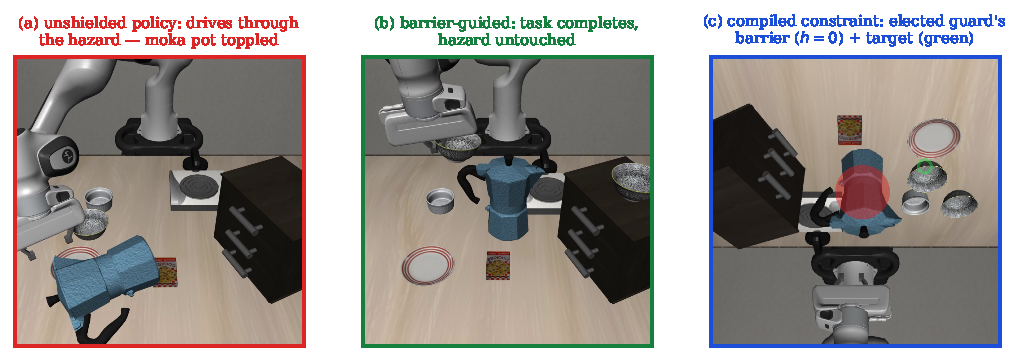
\includegraphics[width=0.80\textwidth]{fig_safelibero.pdf}
\caption{\textbf{From elected hazard to compiled barrier} on a single SafeLIBERO scene. (a) The unguided policy drives through the hazard and topples the moka pot. (b) The same frozen weights under barrier-guided noise-space search complete the task with the hazard untouched. (c) The compiled constraint, showing the elected guard's barrier surface ($h{=}0$) together with the sanctioned target in green. Nothing in this figure is authored per scene; the surface is compiled from the entity that Eq.~\eqref{eq:fol} elects.}
\label{fig:sl}
\end{figure*}

Fig.~\ref{fig:sl} shows the mechanism on one scene, from elected hazard to compiled barrier. Table~\ref{tab:board} places five architectures on identical footing. The post-hoc row is unguided denoising followed by one exact projection of the final chunk, and the reimplementation row is our faithful re-run of the method class of~\cite{sota2607}, using $K{=}1$, a uniform schedule, privileged state, and translational correction, scored under our criterion.\footnote{The task-success uplift of the reimplementation over the baseline reproduces, reaching $+17$ percentage points at Spatial L2, but its published collision-avoidance figure does not reproduce at any swept obstacle radius under a criterion of $>$1\,mm, where the best L2 collision avoidance we obtain is 70.5 and comes at the cost of collapsing L1 task success to 49.0. Their evaluation scores collisions ``by the terminal position of objects'' with no disclosed threshold, whereas ours flags displacement greater than 1\,mm at any timestep. We conclude that the published number rests on a looser or terminal-only criterion, and we therefore present the comparison as one between our system and our own reimplementation.}

We draw three findings from this table. First, post-hoc shielding and in-denoising repair differ by at most 10.5 points of task success and 8.5 points of collision avoidance on any cell, so moving the repair inside the denoising loop is not by itself the source of the improvement. The axis that matters is repair versus search (Sec.~\ref{sec:intro}), not the point in the pipeline at which the repair occurs. Second, the long-horizon liveness stall afflicts every barrier-class shield, with post-hoc shielding scoring 27.5 against a baseline of 58.0, and raising the step cap does not help, whereas our system recovers 15--19 points of task success while doubling collision avoidance. Third, the result most relevant to this workshop appears in the last column: with no privileged state at all, symbolic election combined with perception dominates both shield architectures on both axes in 4 of 8 cells, and achieves parity in task success with 2--5 times the collision avoidance in two further cells.

\subsection{LIBERO-Safety: porting the rule without tuning it}
\label{sec:ls}

\begin{table}[t]
\centering
\caption{LIBERO-Safety, safety-finetuned \pifive{}, TSR/violation\%, paired seeds, $n{=}300$--750 per cell. Violations use the benchmark's own \texttt{:constraints} predicates. Two of the four violation columns carry no information and are marked rather than printed as zeros. The human-safety column is marked \texttt{--} because its sole predicate cannot fire (Sec.~\ref{sec:defect}), and the affordance column is marked \texttt{n/a} because those task files declare no \texttt{:constraints} block at all. That suite expresses safety through its goal predicate, requiring the robot to grasp the handle rather than the blade, so there is nothing to violate by construction. The two obstacle columns are live but measure only the object--hazard half of their conjunction. Macro TSR is unaffected throughout, since task success is scored by the goal predicate.}
\label{tab:ls}
\setlength{\tabcolsep}{2pt}
\small
\begin{tabular}{lccccc}
\toprule
Arm & Obst. & Human & Obst+hand & Afford. & Macro TSR \\
\midrule
Baseline        & 73.6/4.7 & 85.8/-- & 69.3/5.3 & 56.7/n/a & 71.4 \\
Post-hoc shield & 75.3/2.7 & 37.3/-- & 46.0/2.0 & 51.3/n/a & 52.5 \\
SOTA-reimpl.    & 70.7/0.7 & 32.7/-- & 48.0/1.3 & 48.7/n/a & 50.0 \\
Ours (Tier-GT)  & \textbf{77.8}/4.2 & 78.7/-- & 63.2/1.9 & \textbf{58.7}/n/a & 69.6 \\
Ours (Percep)   & 68.7/\textbf{0.7} & \textbf{86.9}/-- & 58.9/1.7 & 56.0/n/a & 67.6 \\
\bottomrule
\end{tabular}
\end{table}

The election rule transfers to a second benchmark without tuning beyond the two class literals already present in Eq.~\eqref{eq:fol}. Table~\ref{tab:ls} reports the five-arm board.

\textbf{Comparison against the two dedicated shields.} Our system improves macro task success by 15--20 points over both shields. On the human suite alone they give up 48--54 task-success points, at $p=1.8\times10^{-16}$ and $p=3.2\times10^{-19}$, while our violation rate matches or undercuts theirs on the two suites where that metric functions. We state these two halves separately by design. The human-suite $p$-values are task-success comparisons, and that suite's violation column is vacuous (Sec.~\ref{sec:defect}), so no safety claim rests upon it. The per-suite pattern is informative: both shields survive the static-obstacle suites and then halve human-safety success, scoring 37.3 and 32.7 against our 86.9. This is the difference between achieving safety by freezing and achieving safety while continuing to move, and it is what the disengage regime provides. Against the unfiltered baseline, our perception-tier violations run 12:1 over 750 paired episodes ($p=0.003$) at task-success parity on three of four suites, and the Tier-GT arm significantly exceeds baseline task success on obstacle avoidance, at 77.8 against 73.6 with $n{=}450$ and $p=0.045$.

\textbf{Results that count against us.} On the obstacle+hand suite our task success is significantly below baseline, at $p=0.005$ and $p=0.03$ depending on tier. This reflects a freeze cost on cells in which the intruder crosses the only viable approach. The baseline's successes on that suite carry a 5.3\% violation rate against our 1.7--1.9\%, which is the trade we are making, but it remains a trade rather than a win.

\textbf{The refusal track.} On the safety-reasoning suite the symbolic judge refuses 100\%, 100\%, and 80\% of unsafe instructions across the three levels, with zero violations, against 80\%, 72\%, and 36\% for the best published model, while the unguided policy executes the same instructions at 94\%, 60\%, and 100\%. This asymmetry between fluent compliance and absent judgment is the representation--action gap of Sec.~\ref{sec:gap} appearing at the level of whole tasks.

\begin{figure*}[t]
\centering
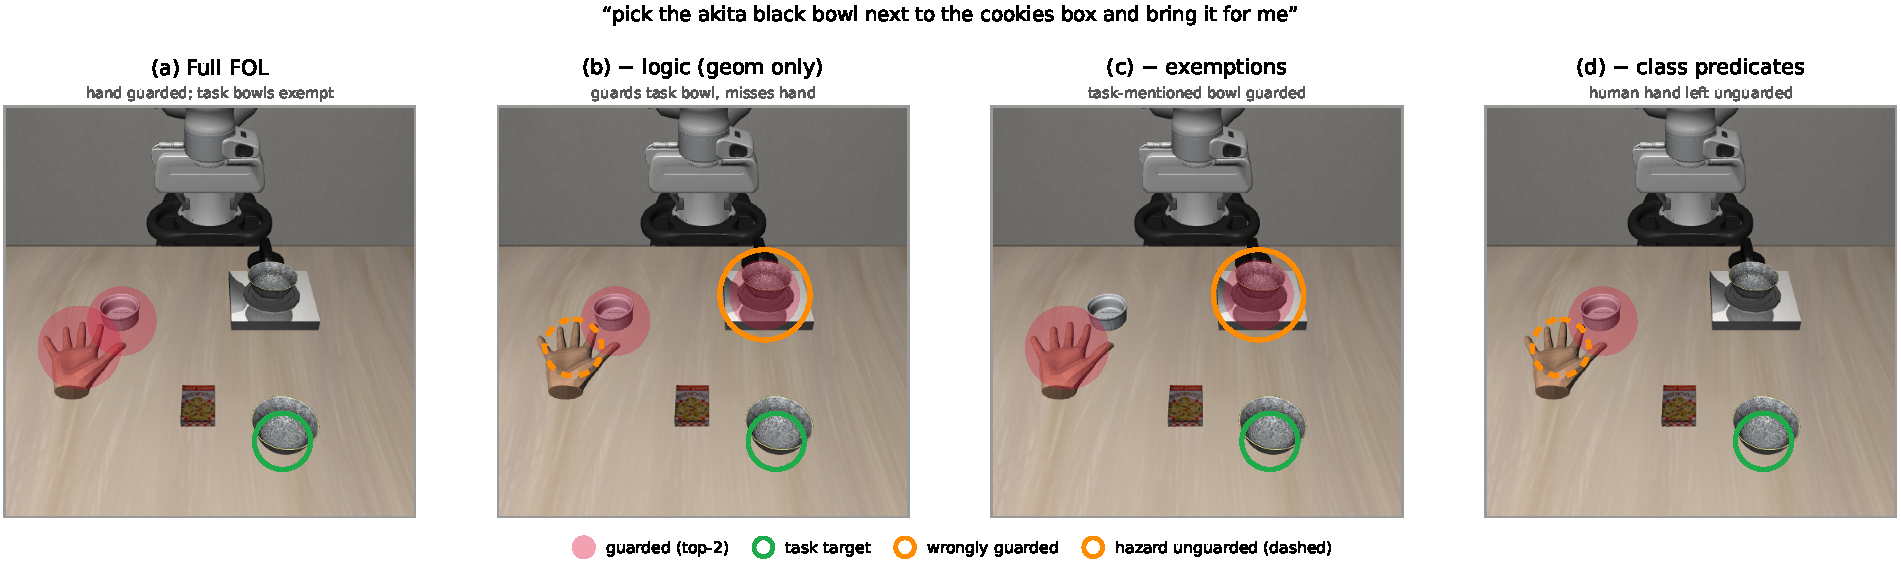
\includegraphics[width=\textwidth]{fig_fol_ablation.pdf}
\caption{\textbf{The contribution of each literal, on a single scene.} Guard sets produced by Eq.~\eqref{eq:fol} under single-clause deletion, for the instruction \textit{``pick the akita black bowl next to the cookies box and bring it for me.''} (a) The full rule guards the human hand and exempts the task bowls. (b) Without the logic, distance ranking guards the task bowl and misses the hand. (c) Without the mention exemptions, the system guards the object it was instructed to pick up and thereby paralyzes itself. (d) Without the class predicates, the hand is left unguarded. Two of the three failures leave the true hazard unprotected, and Table~\ref{tab:ablation} reports the corresponding rollout cost.}
\label{fig:ablation}
\end{figure*}

\subsection{Every literal earns its place}
\label{sec:ablation}

\begin{table}[t]
\centering
\caption{Single-clause deletion from Eq.~\eqref{eq:fol}. Each arm deletes exactly one clause with everything else paired 1:1 on identical initial states, $n{=}150$/cell; exact McNemar. TSR (\%), with violation~\% shown only where it moves. The incumbent column is recomputed on the paired subset, so it differs slightly from Table~\ref{tab:ls}.}
\label{tab:ablation}
\setlength{\tabcolsep}{3pt}
\footnotesize
\begin{tabular}{@{}llccl@{}}
\toprule
Deleted clause & Suite & Full & Ablated & $p$ \\
\midrule
all logic          & Obst.     & 68.7\,{\scriptsize(0.7)} & 44.0\,{\scriptsize(\textbf{4.7})} & 1.2e--6 \\
\;\;(guard nearest-$k$) & Obst+hand & 56.0 & 39.3 & 2.5e--4 \\
                   & Human     & 88.7 & 68.7 & 5.3e--6 \\
\midrule
$\lnot\textsc{Mentioned}$   & Obst.     & 68.7 & 40.0 & 1.8e--8 \\
\;\;exemptions     & Obst+hand & 56.0 & 39.3 & 6.2e--4 \\
\midrule
$\textsc{Prot}\vee\textsc{Mov}$ & Human & 88.7 & 82.0 & 0.10 \\
abstention         & Afford.   & 56.0 & 42.7 & --- \\
VLM property gnd.  & Afford.   & 56.0 & 47.3 & --- \\
\bottomrule
\end{tabular}
\end{table}

This experiment addresses the natural objection that the barrier machinery performs all of the work and the logic is decorative. Fig.~\ref{fig:ablation} shows what each clause supports on a single scene, and Table~\ref{tab:ablation} deletes one clause at a time and measures the resulting rollout cost. Every significant arm confirms its pre-registered prediction, and one result deserves particular emphasis: geometry alone is not merely weaker, it is less safe. Guarding the top-$k$ objects nearest to the path, with no logic at all, raises violations from 0.7\% to 4.7\% ($p=1.2\times10^{-6}$), which is the only arm in the paper that moves violations in the wrong direction, because distance ranking evicts the true hazard from the guard set in favor of a closer but irrelevant object. The mention exemptions are worth approximately 29 task-success points, since without them the system paralyzes itself against its own target. Abstention is worth approximately 13 points, because when the property predicate elects nothing, guarding nothing is preferable to force-electing. Finally, replacing vision-language-grounded property tokens with hand-coded ones costs 8.7 points on the affordance suite, which is the one place where the open vocabulary of the neural component performs measurable work.

\begin{figure}[t]
\centering
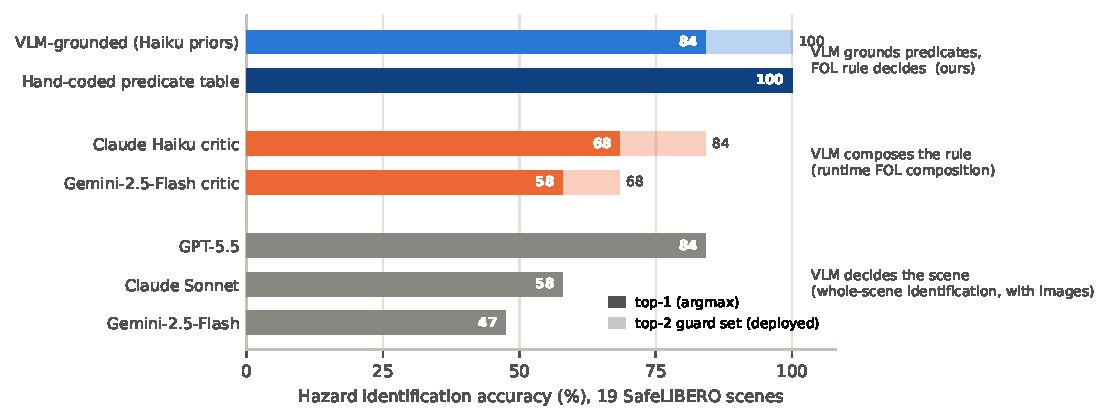
\includegraphics[width=\columnwidth]{fig_vlm_id_accuracy.pdf}
\caption{\textbf{How much authority should the neural component have?} Hazard-identification accuracy on the same 19 SafeLIBERO scenes, grouped by what the VLM is asked to do. Letting it \emph{decide the scene} (grey) or \emph{compose the rule} (orange) is worse than restricting it to \emph{grounding predicates} that a fixed rule composes (blue). Light extensions are the deployed top-2 guard set. The ordering, not any single bar, is the finding.}
\label{fig:vlmauth}
\end{figure}

\subsection{More neural authority fails, and fails unsafe}
\label{sec:negative}

We implemented, pre-registered, and rejected both natural escalations of vision-language authority. These results are what make the division of labor a finding rather than a preference.

\textbf{Learned safety critics, in which prediction was never the bottleneck.} We trained a consequence critic to predict, from the current observation and a candidate action chunk, whether that chunk leads to hazard contact. This corresponds to the second family identified in Sec.~\ref{sec:intro}. Its offline performance is strong, with contact AUC of 0.93--0.999 and end-effector path prediction 8--25 times more accurate than the single-integrator model that our barrier assumes. Converting that predictive accuracy into constrained selection over the $K$ decoded candidates nonetheless produces no rollout gain. On SafeLIBERO Spatial L1, at $n{=}200$ and the privileged tier, critic selection scores 64.5 task success and 28.5 collision avoidance, against 67.5 and 33.8 for the geometric method it was intended to replace and 67.0 and 14.0 unguided, placing it below both references on both axes. On LIBERO-Safety obstacle avoidance the composed critic scores 67.3 against 79.3 for a ten-line geometric engagement gate targeting the identical failure mode. The explanation is informative. In 74.5\% of replans the feasible set is empty and the certified fallback carries the safety in any case, so selection pressure is too weak to matter, and given marginal ranking quality, with a Spearman correlation of 0.597, ranking on every step is net negative. A critic that predicts consequences accurately still requires a set of alternatives to select among, and at this data scale the symbolic gate supplies more decision value than the learned one.

\textbf{Whole-scene VLM identification.} Fig.~\ref{fig:vlmauth} places all three levels of neural authority on one axis, over the same 19 SafeLIBERO scenes. Presenting the whole scene together with its images to an API-strength vision-language model and asking it to name the hazard yields 84.2\% for GPT-5.5, 57.9\% for Claude Sonnet, and 47.4\% for Gemini-2.5-Flash, against 100\% for the decomposed rule. This is the configuration most favourable to the baseline, since images are provided and the strongest available models are used, and the decomposition claim survives it.

\textbf{Runtime composition of the rule by a vision-language model.} Allowing a vision-language model to compose the rule from a predicate library is strictly worse than the fixed rule, using real critics from two vendors. Top-1 and top-2 accuracy over 19 scenes is 13 and 16 for Haiku and 11 and 13 for Gemini, against 16 and 19 for the fixed rule operating over vision-language-grounded predicates. Even with oracle grounding, the entire compositional apparatus gains at most one scene and loses one to selection brittleness. The characteristic failure is the dangerous one, namely over-restrictive conjunctions that fire on nothing, occurring in 2 and 10 empty-rule scenes respectively and leaving the true hazard unguarded. A composition system that failed closed would merely be conservative, whereas this one fails open.

\textbf{Scene graphs, rejected on three separate tests.} Graph-structured identification exactly ties the flat scorer wherever hazards are objects, with 19/19 agreement on SafeLIBERO, and collapses identically on the relational human suite, at 0/2, where the effective fix was instead a ten-line $\textsc{Protected}$ class rule achieving 12/12. Structure was not the missing ingredient; a class predicate was.

\section{A Benchmark Reliability Finding}
\label{sec:defect}

We close with a defect that we did not set out to find. It surfaced because two of our own measurements, taken on the same checkpoint and the same scenes, disagreed. An independent geom-level scorer found 32.0\% robot--hand contact on the human-safety suite, while the benchmark's own violation metric reported 0\% for every arm, including ours and the baselines.

The cause is in \texttt{check\_robot\_contact}, which collects the robot's geoms as integer \emph{indices},
\begin{center}\small\texttt{g\_group.append(geom\_i)}\end{center}
and passes them to \texttt{\_check\_contact}, which tests membership by \emph{name}:
\begin{center}\small\texttt{c1\_in\_g1 = geom\_1\_name in geoms\_1}\end{center}
A string is never a member of a list of integers, and both disjuncts of the acceptance test require a term drawn from that list, so the function returns \texttt{False} unconditionally. \texttt{CheckRobotContact} has therefore never fired, in any suite, for any method evaluated on this benchmark. We supply a standalone executable proof that requires no simulator. A fake contact buffer in which a group-0 gripper geom and the hazard geom touch, in both orderings, returns \texttt{False} as shipped and \texttt{True} when indices are replaced by names. The fix is that single substitution. The defect is isolated, since the object--object \texttt{CheckContact} path and the gripper-part predicates pass names and are correct, and it is specific to this benchmark, which introduced the predicate.

\textbf{The cost of this defect to our own claims.} Our LIBERO-Safety violation numbers measure object--hazard contact only. The sole constraint of the human-safety suite is \texttt{CheckRobotContact}, so its violation rate is identically zero by construction, which is why that column is marked in Table~\ref{tab:ls}. Any reading of the form that the baseline never touches the hand, and that the trained behavior is therefore already safe, is an artifact of the defect. We held that reading ourselves, and we retract it here. The disengage regime remains motivated, but by the genuine collapse in task success under a keep-out region, from a baseline of 54, 56, and 26 to a range of 2--26\%, rather than by a zero-violation baseline. Our macro violation rates average over a structurally zero column and are diluted accordingly, and the 12:1 paired violation result is carried by the remaining three suites. SafeLIBERO is unaffected, since its criterion is ground-truth hazard displacement, computed independently of these predicates. Re-scoring our stored rollouts under the corrected predicate requires per-step contact traces that we did not log, and is the first experiment we intend to run.

\textbf{The relevance of this finding to the present workshop.} This is the third independent defect that we have found in a single safety benchmark, alongside a 25\,cm shift in obstacle spawn position between twin variants that moves the dependent variable, and an unparseable goal predicate that silently zeroes three tasks. Each is a small piece of unchecked imperative code placed where a safety-critical decision is made. The argument for expressing such decisions in a small, inspectable, and individually testable symbolic form is therefore an empirical one rather than an aesthetic one. Every clause of a three-literal rule can be deleted and measured, and we found the failure modes of ours by doing so, whereas a predicate buried in a benchmark's contact-checking utility remained undetected for as long as it has existed.

\section{Limitations}
\label{sec:limitations}

\textbf{Disclosures.} All SafeLIBERO comparisons against the state-of-the-art method are made against our own faithful reimplementation under a single criterion, because the published collision figure does not reproduce under ours at any swept radius. All LIBERO-Safety claims are paired against our self-run baseline on the released checkpoint. That checkpoint reproduces the benchmark's protocol mechanics in our harness but scores well below the published obstacle-avoidance numbers, the release carries no model card, and we were unable to resolve its provenance. The lexicon of the refusal judge was written against the vocabulary of this suite, so its F1 should be read as an in-domain upper bound. The perception tier consumes the symbolic object name list, and removing it costs identification accuracy, reducing top-2 recall from 19 to 12 of 19, so pixel-only naming remains future work.

\textbf{Structural limitations.} Obstacle-on-grasp geometry resists every hard mechanism that we tried, and the 50\% achieved by the soft repulsor is the current ceiling. Identity errors fail unsafe at $k{=}1$, which the guard-set mode mitigates but does not remove. Rotation is uncertified. We extract part-level semantics, distinguishing blade from handle, but ground barriers at the object level, because part perception fails our pre-registered side-discrimination gate. The semantic layer is therefore ahead of what perception can ground, which we regard as the most interesting obstacle to the next version of this system. Divergence between our hazard model and the benchmark definition is real and is visible in Table~\ref{tab:board}, since a semantically correct hazard model can disagree with a benchmark's designated label.

\textbf{Toward hardware.} Our margins are tuned to simulation-grade localization, with 3.6--6.7\,cm median error. The obstacle-motion assumption bounds moving objects at 8\,cm/s or less at 20\,Hz, which is below natural hand speeds, and tracking error is absorbed into the safety margin rather than proved for a specific controller. None of these is an obstacle in principle, and all three remain unproved here.

\section{Conclusion}

All four modules of a safety filter presuppose that someone has named the hazard. For frozen VLA policies, naming the hazard is the difficult part, and it is neither elicitable from the policy nor installable by prompting. The hazard is linearly decodable at the action interface at AUC 0.998, in a policy that cannot answer whether there is a table in front of it and that 98 cells of instruction rewriting cannot redirect. Our response is a division of labor in which neural components ground local, checkable predicates and a fixed three-literal rule makes every safety-critical decision. We defend that division by deleting each literal and measuring what breaks, and by showing that both means of granting the neural component more authority fail unsafe. The fact that this paper had to retract one of its own claims because a benchmark's central safety predicate silently returns false is not incidental to that argument. It is an instance of it.

\section*{Reproducibility}
The standalone proof of the \texttt{CheckRobotContact} defect runs in isolation with no simulator, GPU, or benchmark installation, and is included with the submission.

\begin{thebibliography}{20}

\bibitem{hsu2024safetyfilter} K.-C.~Hsu, H.~Hu, and J.~F.~Fisac, ``The safety filter: A unified view of safety-critical control in autonomous systems,'' \emph{Annual Review of Control, Robotics, and Autonomous Systems}, 2024.

\bibitem{ames2019cbf} A.~D.~Ames et al., ``Control barrier functions: Theory and applications,'' in \emph{European Control Conference (ECC)}, 2019.

\bibitem{mitchell2005hj} I.~M.~Mitchell, A.~M.~Bayen, and C.~J.~Tomlin, ``A time-dependent Hamilton-Jacobi formulation of reachable sets for continuous dynamic games,'' \emph{IEEE Transactions on Automatic Control}, vol.~50, no.~7, 2005.

\bibitem{ames2017cbf} A.~D.~Ames, X.~Xu, J.~W.~Grizzle, and P.~Tabuada, ``Control barrier function based quadratic programs for safety critical systems,'' \emph{IEEE Transactions on Automatic Control}, vol.~62, no.~8, 2017.

\bibitem{bastani2021shielding} O.~Bastani, ``Safe reinforcement learning with nonlinear dynamics via model predictive shielding,'' in \emph{American Control Conference (ACC)}, 2021.

\bibitem{agrawal2017dcbf} A.~Agrawal and K.~Sreenath, ``Discrete control barrier functions for safety-critical control of discrete systems with application to bipedal robot navigation,'' in \emph{Robotics: Science and Systems (RSS)}, 2017.

\bibitem{nakamura2025latent} K.~Nakamura, J.~Seo, and A.~Bajcsy, ``Uncertainty-aware latent safety filters for avoiding out-of-distribution failures,'' arXiv:2505.00779, 2025.

\bibitem{anysafe} S.~Agrawal, J.~Seo, K.~Nakamura, R.~Tian, and A.~Bajcsy, ``AnySafe: Adapting latent safety filters at runtime via safety constraint parameterization in the latent space,'' arXiv:2509.19555, 2025.

\bibitem{nakamura2025latentcbf} K.~Nakamura and A.~Bajcsy, ``How to train your latent control barrier function: Smooth safety filtering under hard-to-model constraints,'' arXiv preprint, 2025.

\bibitem{sota2607} W.~English, H.~Zheng, and R.~Ewetz, ``Neuro-symbolic safety guidance for vision-language-action models via constrained flow matching,'' arXiv:2607.01378, 2026.

\bibitem{liberosafety} Anonymous, ``LIBERO-Safety: Benchmarking safety-aware manipulation for vision-language-action models,'' arXiv:2606.23686, 2026.

\bibitem{yourmodel} Anonymous, ``Your model already knows: Attention-guided safety filter for vision-language-action models,'' arXiv:2606.09749, 2026.

\bibitem{pacs} Anonymous, ``From demonstrations to safe deployment: Path-consistent safety filtering for diffusion policies,'' arXiv:2511.06385, 2025.

\bibitem{vls} Anonymous, ``VLS: Steering pretrained robot policies via vision-language models,'' arXiv:2602.03973, 2026.

\bibitem{frs} Anonymous, ``Improving robotic generalist policies via flow reversal steering,'' arXiv:2606.13675, 2026.

\bibitem{safediffuser} W.~Xiao et al., ``SafeDiffuser: Safe planning with diffusion probabilistic models,'' arXiv:2306.00148, 2023.

\bibitem{aegis} Anonymous, ``AEGIS: A geometric safety shield for vision-language-action policies,'' arXiv:2512.11891, 2025.

\bibitem{brunke2025semantic} L.~Brunke et al., ``Semantically safe robot manipulation: From semantic scene understanding to motion safeguards,'' \emph{IEEE Robotics and Automation Letters}, 2025.

\bibitem{vlasurvey} Anonymous, ``Vision-language-action safety: Threats, challenges, evaluations, and mechanisms,'' arXiv:2604.23775, 2026.

\bibitem{gdino} S.~Liu et al., ``Grounding DINO: Marrying DINO with grounded pre-training for open-set object detection,'' in \emph{ECCV}, 2024.

\bibitem{pi05} Physical Intelligence, ``$\pi_{0.5}$: A vision-language-action model with open-world generalization,'' arXiv:2504.16054, 2025.

\end{thebibliography}

\end{document}
